\documentclass{article}

\usepackage{color}
\usepackage{graphicx}
\usepackage{tabularx}


\usepackage{geometry}
 \geometry{
 top=20mm,
 bottom=20mm,
 }


\title{Document pour l'adapation des interfaces}
\author{Justal Kevin}
\date{28/09/2015}
\renewcommand{\contentsname}{Table des mati\`eres} 
 
\newcommand\invisiblesection[1]{%
  \refstepcounter{section}%
  \addcontentsline{toc}{section}{\protect\numberline{\thesection}#1}%
  \sectionmark{#1}} 
 
\begin{document}

\begin{center}
\textbf{\Huge{Bootstrap contre Polymer}}
\line(1,0){300}\\
DOSSIER D'ANALYSE DES DIFFERENCES\\
\vspace{3cm}
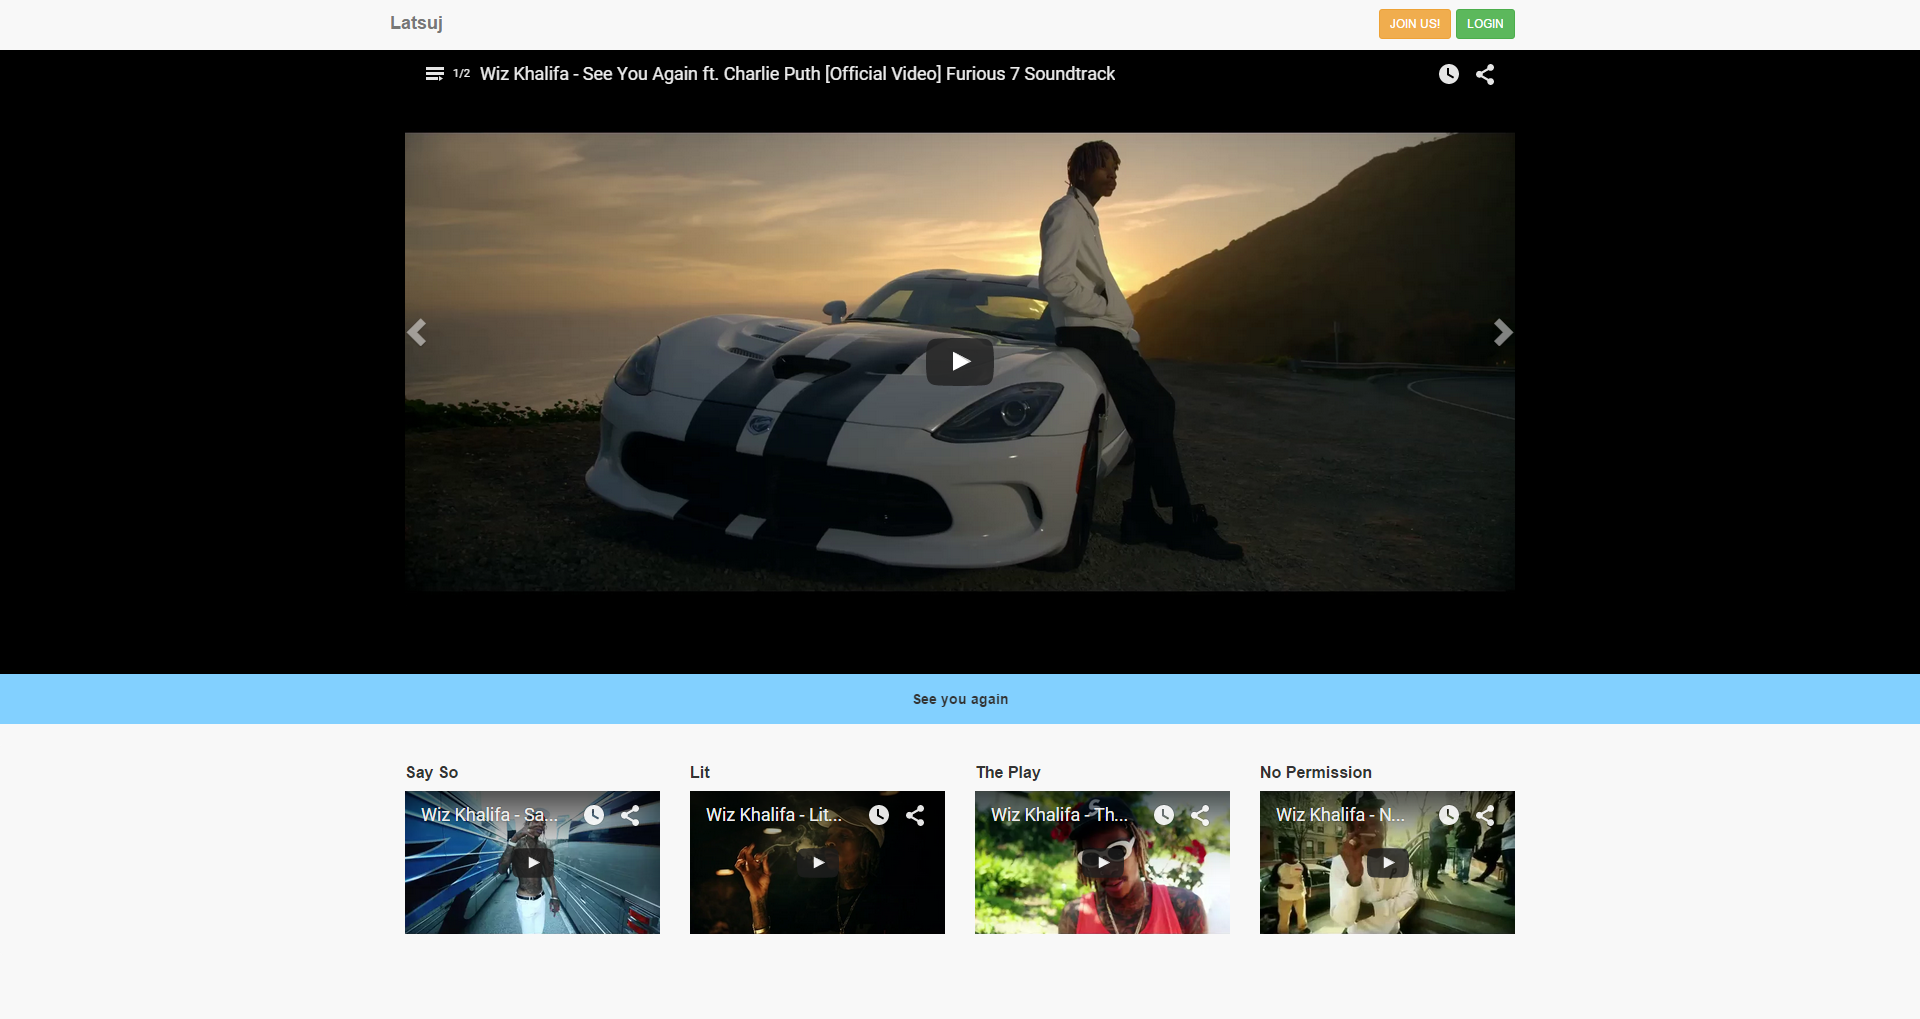
\includegraphics[width=1.0\textwidth]{pc}\\
\vspace{3cm}
\textbf{\Large{JUSTAL KEVIN}}\\
2015\\
\vspace{2cm}
\textbf{Justal Kevin - \color{blue}{\underline{justal@polytech.unice.fr}} \color{black}{- SI5 - IHM}}\\
\vspace{4cm}
\textbf{Enseignant :}\\
\textbf{Anne Marie Dery - \color{blue}{\underline{dery@polytech.unice.fr}}}
\end{center}

\newpage
\newpage
\tableofcontents

\newpage

\section{Site Web Adaptatif}

Le site a \'et\'e pens\'e sur le principe du RWD (\textit{responsive web design}) ou site web adaptatif dans la langue de mol\'ere. Ce concept s'appuit sur l'usage des \textit{Media queries}, des grille ou encore des images flexibles. Au fur et \`a mesure que nous creuserons les deux frameworks, nous verrons que Polymer s'appuie principalement sur les media queries tandis que Boostrap lui, poss\'ede en plus un syst\`eme de grille tr\`es utile. 
\vspace{0.5cm}\\
Pour d\'evelopper, je suis parti de la version ordinateur, puis j'ai remis en forme les \'el\'ements \`a mesure que la largeur de l'\'ecran diminuait voire je les supprimais. Nous verrons un peu plus loin pourquoi j'ai choisi de supprimer des \'el\'ements.
\begin{center}
\vspace{0.5cm}
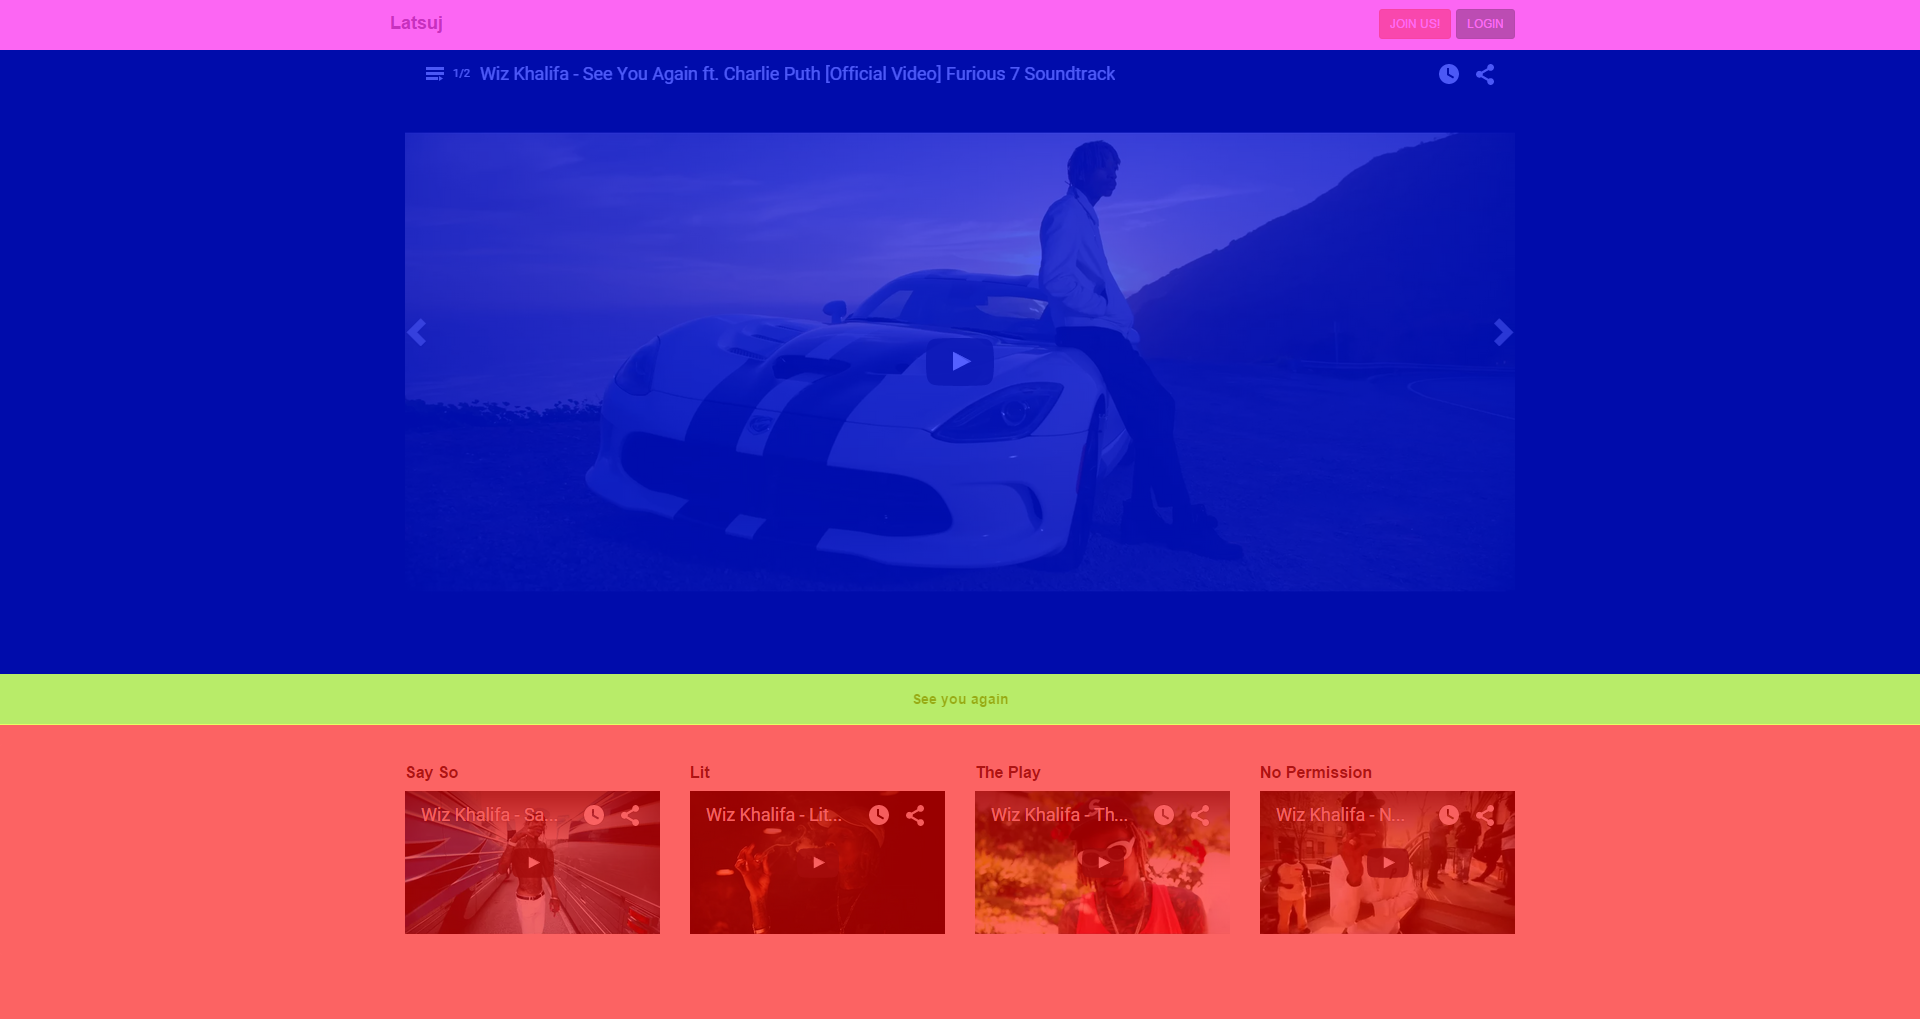
\includegraphics[width=0.8\textwidth]{pc2}
\vspace{0.5cm}
\end{center}

Le site a un d\'ecoupage en quatre grands blocs. En rose sur l'image ci-dessus, on trouve la barre de connexion. En bleu, la zone de visionnage des vid\'eo. En Jaune, une zone d'information. Enfin, en rouge, une zone pour afficher les vid\'eos o\`u le chanteur est le m\^eme que la vid\'eo dans la zone bleu.\\
Pour observer pr\'ecis\'ement le principe de RWD, nous allons nous int\'erresser particuli\`erement \`a la zone rouge en bas du site. Cette derni\'ere illustre \`a la perfection tous les aspects que l'on attend d'un site adaptatif. Colorions chaque divisions de cette partie du site d'une couleur unique.
\begin{center}
\vspace{0.5cm}
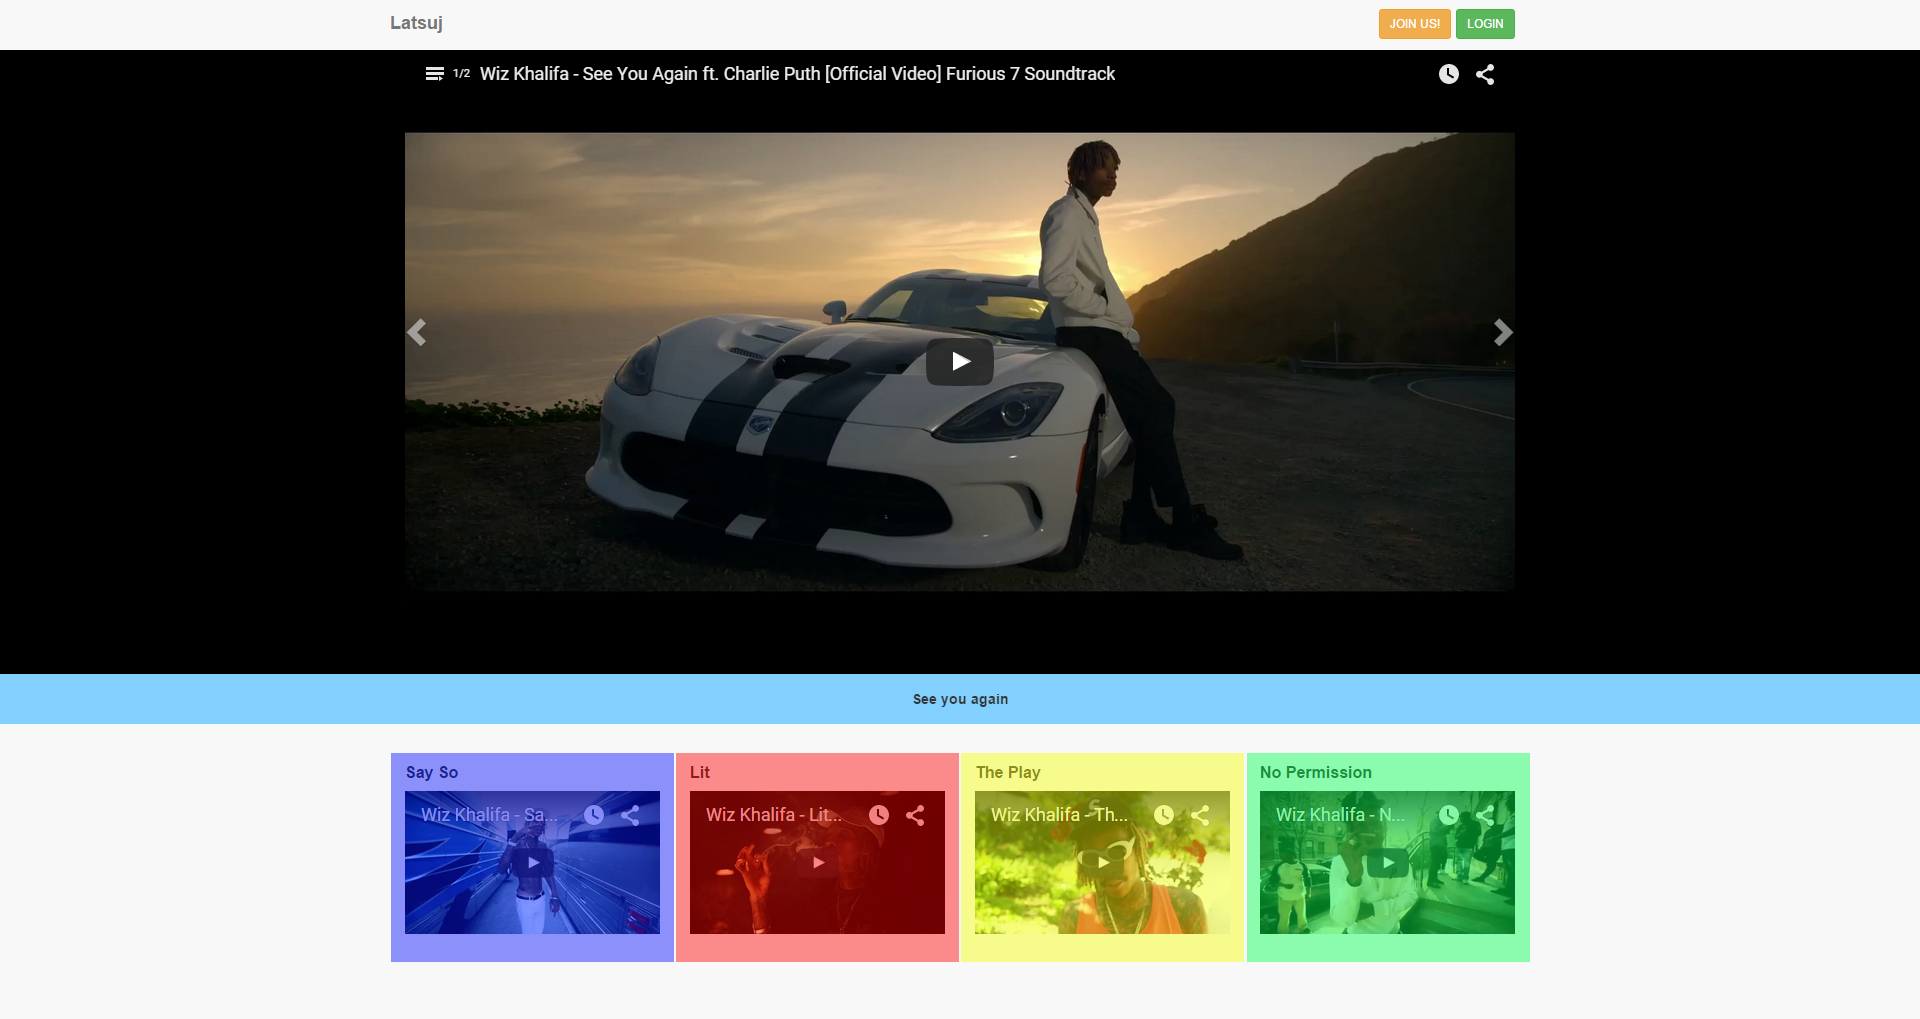
\includegraphics[width=0.8\textwidth]{pc4}
\vspace{0.5cm}
\end{center}
Si nous r\'eduisons la largeur de la fenetre, le contenu s'adaptera. Dans un premier temps, il n'y aura plus que deux blocs par ligne. Puis, si nous continuons de r\'eduire la fen\`etre, il n'y aura plus qu'un seul bloc par ligne et les deux derniers auront \'et\'e cach\'e.
\begin{center}
\vspace{0.5cm}
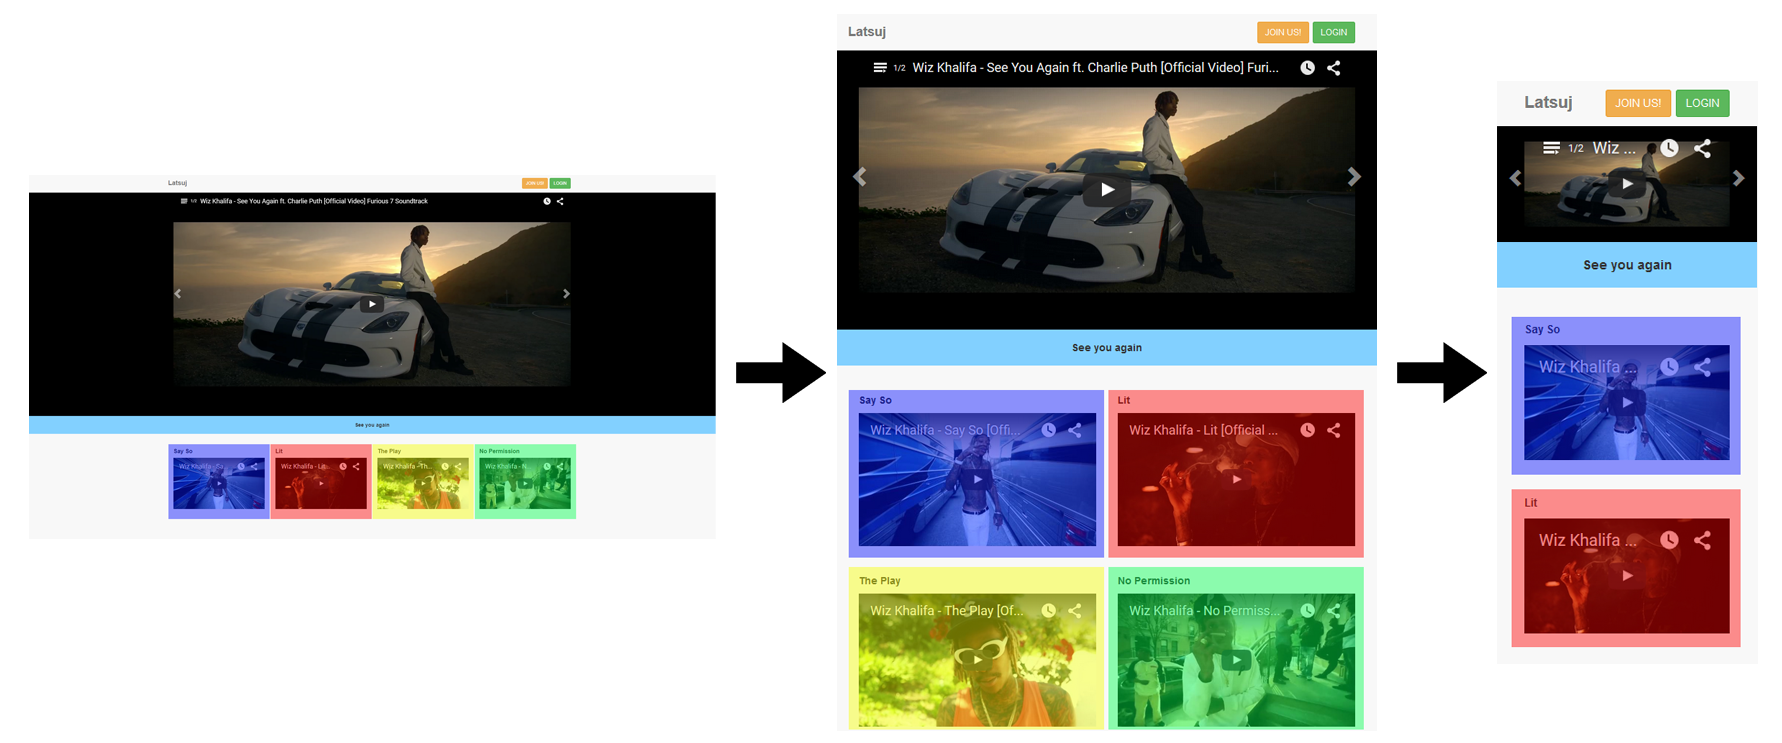
\includegraphics[width=0.8\textwidth]{pc7}
\vspace{0.5cm}\\
\end{center}

Le site s'adapte donc aux dimensions de notre appareil ou fen\`etre.\`A quoi cela peut-il bien servir ? Il serait plus adapté de se demander quels sont probl\`emes que cela r\'esout-il ? Comme on le voit autour de nous, les ordinateurs ne sont plus les seuls \'el\'ements ou gadgets nous entourant, ils existent maintenant une innombrable quantit\'e d'apareil informatique de tous types et de toutes dimensions. Il est important qu'un site internet ne laisse aucun utilisateur sur le bas cot\'e. Comme il est impensable de concevoir une application ou un site internet pour chaque appareil, il faut donc faire un site qui puisse s'adapter suivant les dimensions de l'appareil. 
\vspace{0.5cm}\\
Mais ce n'est pas tout, l'adaptation seul ne permet pas d'\'etablir ce que l'on peut appeler un site web adaptatif. Le cr\'eateur de cette vision, Mr. Ethan Marcotte, a implement\'e un site (\textit{http://alistapart.com/d/responsive-web-design/ex/ex-site-flexible.html}) qui s'adapte \`a la largeur de l'\'ecran. Cependant, il pointe du doigt certains d\'etails. Par exemple, lorsque l'on redimensionne la page, les \'el\'ements vont bel et bien se redimensionner mais les images et le texte \`a tr\`es basse r\'esolution deviendront illisible. Il faut donc que les \'el\'ements se repositionnent dans la page afin que le contenue soit lisible et agr\'eable \`a arpenter pour l'utilisateur.\\

Le site est aussi \textit{responsible typesetting}. La taille en pixel du texte varie suivant la taille de la fen\`etre. Pour l'utilisateur, il est sans aucun doute plus agr\'eable de pouvoir lire les paroles d'une chanson phrase par phrase. Or, si la taille du texte restait la m\^eme pour toutes dimensions de fen\`etre, soit le texte serait illisible \`a une grande r\'esolution, soit le site serait incommode \`a basse r\'esolution. Pour r\'esoudre ce probl\`eme, une proportions a \'et\'e sp\'ecifier pour l'ensemble des textes suivant la largeur de la fen\`etre ou de l'appareil.\\

Fitt's law

\section{Boostraps}


\section{Documentations, Outils, liens utiles} 

\textbf{Ethan Marcotte}\\
\textit{http://alistapart.com/d/responsive-web-design/ex/ex-site-flexible.html}\\
\textit{http://alistapart.com/d/responsive-web-design/ex/ex-site-linearize.html}\\

\textbf{Responsible typesetting}
\textit{http://blog.line0.eu/responsible-typesetting/}




\section{Difficult\'es rencontr\'es}
\hspace*{0.6cm}Le premier probl\`eme rencontr\'e fut lorsque que j'essaya de coder une balise div de telle mani\`ere que celle-ci remplisse enti\`erement l'espace de l'application. Cette chose extr\`emement simple n'est pourtant pas impl\'ement\'e dans Bootstrap 3.0 et les versions sup\'erieur alors que cela se trouvait dans les versions ant\'erieur avec la class span. Apr\'es de longue recherches, il apparait donc impossible en pur Bootstrap de remplir un div \`a cent pour cent de la balise parent.De ce fait, j'ai du modifi\'e le CSS pour r\'ealiser le remplissage de la page. Pourquoi un tel choix des d\'eveloppeur de bootstrap ?

margin-bottom : Seriously ?

Compatibilite : WTF polymer !

min-height ? WTF do not work !OK parce que tous ces putain d'elements sont en inline et non en block...Ok l'erreur

Suivre un ordre pour appeler les modules au depart, les enfant en premier.

encapsulation des elements ? content :X Merci la doc....pourrie.

Le carousel une horreur sur Polymer....

\section{Simple trouvaille d'optimisation}
En farfouillant sur les documentations de Bootstrap, je suis tomb\'e sur une optimisation qui a retenu mon attention. Une chose simple et pourtant efficace que je ne faisait pas moi non plus. Les developpeurs de Bootstrap mettent toujours les scripts javascript en fin de page afin d'accelerer le chargement de la page. Cela peut paraitre stupide comme remarque mais je tiens \`a m'en souvenir, j'en fait donc par dans mon document.

Petite astuce, enlever les ; sur le dernier elements de css pour gagner un caractere de lecture.

\end{document}
